

\tikzset{every picture/.style={line width=0.3pt}} %set default line width to 0.75pt        

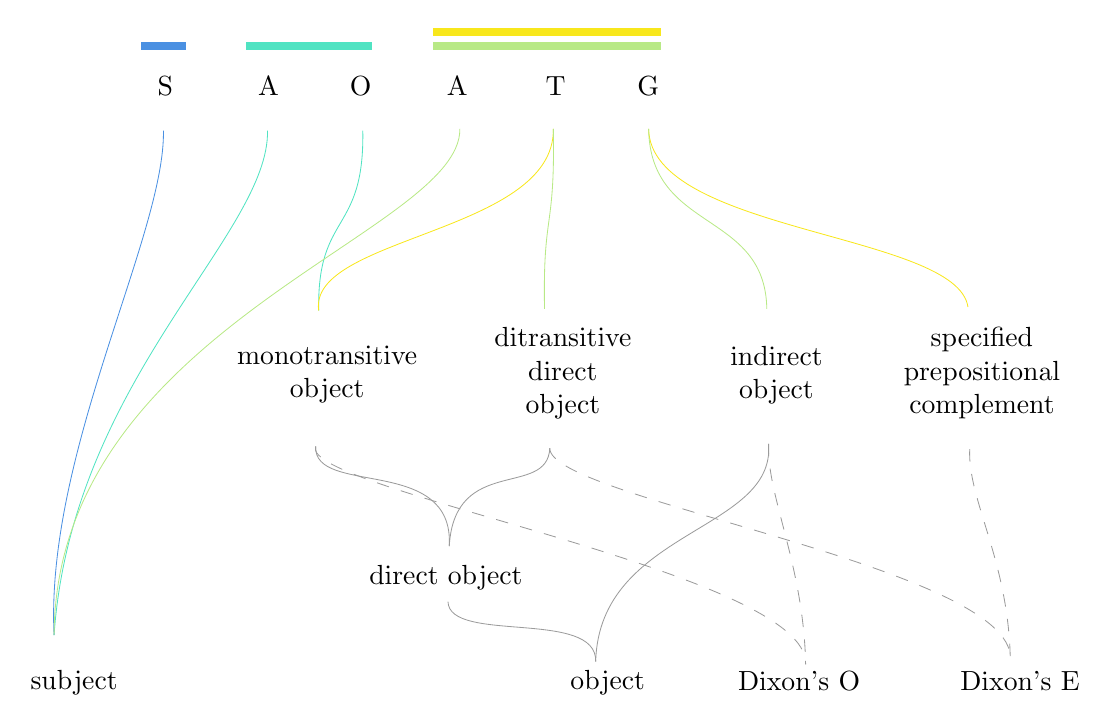
\begin{tikzpicture}[x=0.75pt,y=0.75pt,yscale=-0.85,xscale=0.85]
%uncomment if require: \path (0,513); %set diagram left start at 0, and has height of 513

%Straight Lines [id:da5590373900481334] 
\draw [color={rgb, 255:red, 74; green, 144; blue, 226 }  ,draw opacity=1 ][line width=3]    (132,62) -- (157.72,62) ;
%Straight Lines [id:da6034249079442651] 
\draw [color={rgb, 255:red, 80; green, 227; blue, 194 }  ,draw opacity=1 ][line width=3]    (191.72,62) -- (262.72,62) ;
%Straight Lines [id:da3340903560309998] 
\draw [color={rgb, 255:red, 184; green, 233; blue, 134 }  ,draw opacity=1 ][line width=3]    (297.72,62) -- (426.72,62) ;
%Curve Lines [id:da7559551700584779] 
\draw [color={rgb, 255:red, 80; green, 227; blue, 194 }  ,draw opacity=1 ]   (257.72,109.97) .. controls (258.72,168.97) and (231.72,155.97) .. (232.72,211.97) ;
%Curve Lines [id:da6470497609004202] 
\draw [color={rgb, 255:red, 80; green, 227; blue, 194 }  ,draw opacity=1 ]   (203.72,109.97) .. controls (204.72,168.97) and (92.72,250.94) .. (82.72,395.94) ;
%Curve Lines [id:da9535821756090674] 
\draw [color={rgb, 255:red, 74; green, 144; blue, 226 }  ,draw opacity=1 ]   (144.72,109.97) .. controls (145.72,168.97) and (77.72,291.94) .. (82.72,395.94) ;
%Curve Lines [id:da4943116446528697] 
\draw [color={rgb, 255:red, 184; green, 233; blue, 134 }  ,draw opacity=1 ]   (312.72,108.97) .. controls (313.72,167.97) and (83.72,220.94) .. (82.72,395.94) ;
%Curve Lines [id:da034641113672127855] 
\draw [color={rgb, 255:red, 248; green, 231; blue, 28 }  ,draw opacity=1 ]   (365.72,108.97) .. controls (366.72,167.97) and (226.72,169.97) .. (232.72,211.97) ;
%Curve Lines [id:da5196681080395307] 
\draw [color={rgb, 255:red, 248; green, 231; blue, 28 }  ,draw opacity=1 ]   (419.72,108.97) .. controls (420.72,167.97) and (594.72,167.97) .. (600.72,209.97) ;
%Straight Lines [id:da23388092728957277] 
\draw [color={rgb, 255:red, 248; green, 231; blue, 28 }  ,draw opacity=1 ][line width=3]    (297.72,54) -- (426.72,54) ;
%Curve Lines [id:da13093524389220645] 
\draw [color={rgb, 255:red, 184; green, 233; blue, 134 }  ,draw opacity=1 ]   (365.72,108.97) .. controls (366.72,167.97) and (359.72,154.97) .. (360.72,210.97) ;
%Curve Lines [id:da2405074684879065] 
\draw [color={rgb, 255:red, 184; green, 233; blue, 134 }  ,draw opacity=1 ]   (419.72,108.97) .. controls (420.72,167.97) and (485.72,154.97) .. (486.72,210.97) ;
%Curve Lines [id:da5399897307832593] 
\draw [color={rgb, 255:red, 155; green, 155; blue, 155 }  ,draw opacity=1 ]   (231,289) .. controls (229.72,317.57) and (309.72,293.57) .. (306.72,345.57) ;
%Curve Lines [id:da43486300562119107] 
\draw [color={rgb, 255:red, 155; green, 155; blue, 155 }  ,draw opacity=1 ]   (363.72,289.94) .. controls (362.43,318.5) and (309.72,293.57) .. (306.72,345.57) ;
%Curve Lines [id:da9115056023887791] 
\draw [color={rgb, 255:red, 155; green, 155; blue, 155 }  ,draw opacity=1 ]   (306,377) .. controls (306.72,400.94) and (390.72,380.94) .. (389.72,410.94) ;
%Curve Lines [id:da27935753858234835] 
\draw [color={rgb, 255:red, 155; green, 155; blue, 155 }  ,draw opacity=1 ]   (487.72,287.57) .. controls (491.72,337.57) and (391.72,335.94) .. (389.72,410.94) ;
%Curve Lines [id:da7115308344150204] 
\draw [color={rgb, 255:red, 155; green, 155; blue, 155 }  ,draw opacity=1 ] [dash pattern={on 4.5pt off 4.5pt}]  (231,289) .. controls (221.72,313.57) and (511.72,360.57) .. (508.72,412.57) ;
%Curve Lines [id:da31095802179111853] 
\draw [color={rgb, 255:red, 155; green, 155; blue, 155 }  ,draw opacity=1 ] [dash pattern={on 4.5pt off 4.5pt}]  (487.72,287.57) .. controls (486.43,316.13) and (507.72,356.57) .. (508.72,412.57) ;
%Curve Lines [id:da630655999182743] 
\draw [color={rgb, 255:red, 155; green, 155; blue, 155 }  ,draw opacity=1 ] [dash pattern={on 4.5pt off 4.5pt}]  (363.72,289.94) .. controls (362.43,318.5) and (627.72,357.57) .. (624.72,409.57) ;
%Curve Lines [id:da5122649297059649] 
\draw [color={rgb, 255:red, 155; green, 155; blue, 155 }  ,draw opacity=1 ] [dash pattern={on 4.5pt off 4.5pt}]  (601.72,290.57) .. controls (600.43,319.13) and (623.72,353.57) .. (624.72,409.57) ;

% Text Node
\draw (140,78) node [anchor=north west][inner sep=0.75pt]   [align=left] {S};
% Text Node
\draw (197,78) node [anchor=north west][inner sep=0.75pt]   [align=left] {A};
% Text Node
\draw (249,78) node [anchor=north west][inner sep=0.75pt]   [align=left] {O};
% Text Node
\draw (304,78) node [anchor=north west][inner sep=0.75pt]   [align=left] {A};
% Text Node
\draw (412,78) node [anchor=north west][inner sep=0.75pt]   [align=left] {G};
% Text Node
\draw (360,78) node [anchor=north west][inner sep=0.75pt]   [align=left] {T};
% Text Node
\draw (68,414.5) node [anchor=north west][inner sep=0.75pt]   [align=left] {subject};
% Text Node
\draw (182,230.75) node [anchor=north west][inner sep=0.75pt]   [align=left] {\begin{minipage}[lt]{68.99pt}\setlength\topsep{0pt}
\begin{center}
monotransitive\\object
\end{center}

\end{minipage}};
% Text Node
\draw (328,220.25) node [anchor=north west][inner sep=0.75pt]   [align=left] {\begin{minipage}[lt]{53.13pt}\setlength\topsep{0pt}
\begin{center}
ditransitive\\direct\\object
\end{center}

\end{minipage}};
% Text Node
\draw (462,230.75) node [anchor=north west][inner sep=0.75pt]   [align=left] {\begin{minipage}[lt]{36.67pt}\setlength\topsep{0pt}
\begin{center}
indirect\\object
\end{center}

\end{minipage}};
% Text Node
\draw (560,220.25) node [anchor=north west][inner sep=0.75pt]   [align=left] {\begin{minipage}[lt]{60.22pt}\setlength\topsep{0pt}
\begin{center}
specified\\prepositional\\complement
\end{center}

\end{minipage}};
% Text Node
\draw (260,355) node [anchor=north west][inner sep=0.75pt]   [align=left] {direct object};
% Text Node
\draw (374,414.5) node [anchor=north west][inner sep=0.75pt]   [align=left] {object};
% Text Node
\draw (469,415) node [anchor=north west][inner sep=0.75pt]   [align=left] {Dixon's O};
% Text Node
\draw (595,415) node [anchor=north west][inner sep=0.75pt]   [align=left] {Dixon's E};


\end{tikzpicture}
